% % % % % % % % % % % % % % % % % % % % % 
% dbi.tex - Ian Huston
% $Id: dbi.tex,v 1.57 2009/10/31 11:18:08 ith Exp $
% % % % % % % % % % % % % % % % % % % % % 
% Redefine CVSRevision for this section
\renewcommand{\CVSrevision}{\version$Id: dbi.tex,v 1.57 2009/10/31 11:18:08 ith Exp $}

% % % % % % % % % % % % % % % % % % % % % % % % % % % % % % % % 
% =========================================================== %
% % % % % % % % % % % % % % % % % % % % % % % % % % % % % % % % 
\chapter{Observational Bounds on DBI Inflation}
\label{ch:dbi}
% % % % % % % % % % % % % % % % % % % % % % % % % % % % % % % % 
% =========================================================== %
% % % % % % % % % % % % % % % % % % % % % % % % % % % % % % % % 
% 
% 
% 
% % % % % % % % % % % % % % % % % % % % % % % % % % % % % % % % 
% =========================================================== %
% % % % % % % % % % % % % % % % % % % % % % % % % % % % % % % % 
\section{Introduction}
\label{sec:intro-dbi}
% % % % % % % % % % % % % % % % % % % % % % % % % % % % % % % % 
% =========================================================== %
% % % % % % % % % % % % % % % % % % % % % % % % % % % % % % % % 

In this chapter two bounds on the amplitude of primordial gravitational waves will be derived, which
severely challenge the standard
DBI inflationary scenario. By considering the field range of observable
inflation inside a warped throat, the tensor-scalar ratio $r$ will be
constrained to be less than $10^{-7}$. In contrast a lower bound of $r\gsim
0.005$ will be derived when the power spectrum of scalar perturbations has a red
spectral index. These clearly incompatible bounds can be relaxed by using a more
general form of the DBI action.

% 
The gravitational wave background generated in DBI 
inflation was initially investigated by Baumann and McAllister (BM) 
\cite{bmpaper}. By exploiting a relationship due originally 
to Lyth \cite{lyth}, these authors derived a field-theoretic upper limit 
to the tensor amplitude and concluded that 
rather stringent conditions would need to be satisfied for these 
perturbations to be detectable.      
Moreover, the special case of 
DBI inflation driven by a quadratic potential is incompatible with the WMAP3 
data when this constraint is imposed \cite{bean}.  


Our aim in this chapter is to derive observational constraints on DBI inflation
that are 
insensitive to the details of the throat geometry and the inflaton potential. 
In general, there are two realizations of the scenario, 
which are referred to as the ultra-violet (UV) and infra-red (IR) 
versions. These are characterized respectively by whether the brane is 
moving towards or away from the tip of the throat. 
We focus initially on the UV scenario 
and derive an upper bound on 
the gravitational wave amplitude in terms of observable 
parameters. This limit arises by considering 
the variation of the inflaton field during the era when 
observable scales cross the Hubble radius, and 
we find in general that the tensor-scalar ratio must satisfy 
$r \, \lsim \, 10^{-7}$. This 
is below the projected sensitivity of future Cosmic Microwave Background (CMB) polarization 
experiments \cite{Baumann:2008aq,vpj}. 

On the other hand, the WMAP5 data 
favours a red perturbation spectrum with 
$n_s<1$ when  
the scalar spectral index is effectively constant \cite{Komatsu:2008hk}. 
For models which generate such a spectrum, 
we identify a corresponding lower limit on the 
tensor modes such that $r \, \gsim \, 0.1 (1-n_s)$. 
This is incompatible with the upper bound 
on $r$ when $1-n_s \simeq 0.03$, as inferred
by the observations. 

Therefore a reconciliation between theory and observation 
requires either a relaxation of the upper limit on $r$ or a blue 
spectral index $(n_s >1)$. The DBI scenario would need 
to be generalized in a suitable way for the upper bound on $r$
to be weakened. Necessary conditions are identified that a 
generalized action must satisfy for the BM constraint and our newly derived
bound to be relaxed. 
Such conditions are shown in Chapter~\ref{ch:multibrane} to be
realized in a recently proposed IR version of DBI inflation driven
by multiple coincident branes \cite{thomasward}. 

% 
% 
% % % % % % % % % % % % % % % % % % % % % % % % % % % % % % % % 
% =========================================================== %
% % % % % % % % % % % % % % % % % % % % % % % % % % % % % % % % 
\section{An Upper Bound on the Primordial Gravitational Waves}
% 
\label{sec:upper-dbi}
% % % % % % % % % % % % % % % % % % % % % % % % % % % % % % % % 
% =========================================================== %
% % % % % % % % % % % % % % % % % % % % % % % % % % % % % % % % 
%

In \Rref{bmpaper} Baumann and McAllister
derived a field-theoretic upper bound on the tensor-scalar ratio. They achieved
this by noting that the four-dimensional Planck mass is related 
to the volume of the compactified CY manifold, $V_6$, such that 
$\Mpl^2=V_6 \kappa_{10}^{-2}$, where $\kappa_{10}^2 \equiv 
\frac{1}{2} (2\pi )^7 g_s^2 m_s^{-8} = \pi /T_3^{2}$ for a 
${\rm D3}$-brane \footnote{We parameterise the Planck scale 
in terms of the ${\rm D3}$-brane tension out of convenience, 
and note that there is no physical relationship between the two.}.
In general, the compactified volume 
is comprised of bulk and throat contributions, 
$V_6 = V_{6,{\rm bulk}}+V_{6,{\rm throat}}$. The latter is 
given by
% 
\begin{equation}
\label{eq:throatvolume}
V_{6,\mathrm{throat}} = \mathrm{Vol}(X_5)  
\int_0^{\rho_{UV}} \d\rho \frac{\rho^5}{h^4(\rho )} \,,
\end{equation}
% 
where $\rho_{UV}$ denotes the radial coordinate at 
the edge of the throat (defined as the region 
where $h (\rho_{UV})$ is of order unity). The geometry of the throat is shown
in Figure~\ref{fig:throat-geom}.

% 
\begin{figure}
 \centering
 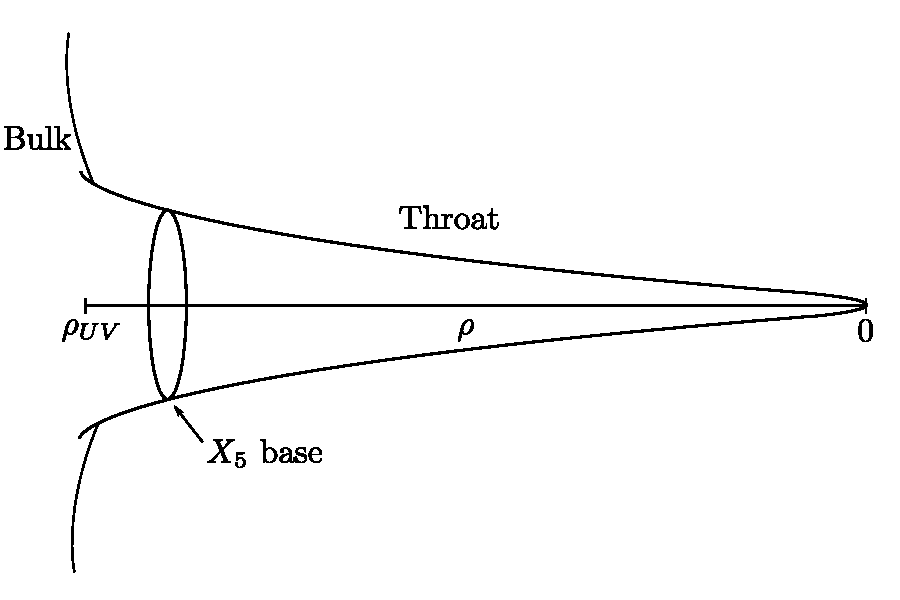
\includegraphics[width=\textwidth]{./dbi/graphs/throat-geom.pdf}
 % throat-geom.pdf: 432x288 pixel, 72dpi, 15.24x10.16 cm, bb=0 0 432 288
 \caption[Warped Throat Geometry]{Geometry of the warped throat. The radial
coordinate $\rho$ is measured from the tip of the throat to $\rho_{UV}$ at the join
with the bulk manifold.}
 \label{fig:throat-geom}
\end{figure}

% 

If one assumes that the bulk volume is 
non-negligible relative to 
that of the throat (i.e. $V_{6,\mathrm{throat}} < V_{6}$), 
it follows that $\Mpl^2> V_{6,\mathrm{throat}}\kappa_{10}^{-2}$. 
For a warped $AdS_5 \times X_5$ geometry, this leads to an 
upper limit on the total variation of the inflaton field in 
the throat region in terms of the D3 charge:
% 
\begin{equation}
\label{eq:BMbound-dbi}
\frac{\varphi_{UV}}{\Mpl}   < \frac{2}{\sqrt{N}} \,.
\end{equation}
% 


Condition (\ref{eq:BMbound-dbi}) may be converted into a 
corresponding limit on the tensor-scalar ratio by noting from 
the definition (\ref{eq:epsdefn-dbiintro})
that $\dot{\varphi}^2 /\Mpl^2 = 2\varepsilon_H H^2/P_{,X}$.
This implies that the variation of the inflaton field 
is given by the Lyth bound \eq{eq:genlyth-dbiintro} 
\cite{lyth,bmpaper}
% 
\begin{equation}
\label{eq:rtheory}
\frac{1}{\Mpl^2} \left( \frac{\d\varphi}{\d \N} \right)^2 =
\frac{r}{8} \,,
\end{equation}
% 
where $\N$ is the number of e-foldings as defined in \eq{eq:nefolddefn-intro}. 
Since $\vp_*$, the field value during observable inflation,  is
less than $\varphi_{UV}$
this results in an upper bound on the observable tensor-scalar ratio
\cite{bmpaper}: 
% 
\begin{equation}
\label{eq:BMboundr}
r_*  < \frac{32}{N (\Neff)^2} \,.
\end{equation}
% 
The effective number of e-foldings $\Neff$, defined in
\eq{eq:Neff-dbiintro}, 
is a model-dependent parameter that quantifies 
how $r$ varies during the final stages of inflation. Since $c_s\PX = 1$ in the
standard DBI model, 
it follows that $\Neff = \N_\mathrm{end}$ if $r$ is constant during inflation,
where $\N_\mathrm{end}$ is the total number of e-foldings
from the epoch of observable inflation until inflation ends.


Typically, one expects $30 \, \lsim \, {\Neff} 
\, \lsim \, 60$, 
although smaller values may be possible if the slow-roll conditions are 
violated after observable scales have crossed the horizon. 
Furthermore, $N \gg 1$ is necessary 
for backreaction effects to be negligible \cite{bmpaper}. 
Hence, the constraint \eqref{eq:BMboundr} 
imposes a strong restriction on DBI inflationary models. 
On the other hand, the numerical value 
of $\Neff$ is uncertain.  
Our aim here is to focus on the range of values covered by the 
inflaton field during the observable stages of inflation. 
This will result in a constraint on the tensor modes that 
can be expressed in terms of observable parameters.  


To proceed, we denote the change in the value of the inflaton field over 
observable scales by 
$\Delta  \varphi _{*} = \sqrt{T_3} \Delta \rho_{*}$. 
Since the brane moves towards the tip of the throat in 
UV DBI inflation, it follows that $\rho_{*} > \rho_{end} >0$, which 
implies that  
% 
\begin{equation}
\label{eq:importantbound}
\rho_{*} > |\Delta \rho _{*}| \,.
\end{equation}
% 
This change in the inflaton value will correspond 
to a fraction of the throat volume, 
$| \Delta V _{6,*}|  < {V_{6,\mathrm{throat}}} \, \lsim \, {V_6} $,
where equality in the second limit arises if
the bulk volume is negligible. Hence, 
$| \Delta \varphi_* |$ is bounded such that  
% 
\begin{equation}
\label{eq:halfwayconstraint}
\left( \frac{\Delta \varphi}{\Mpl} \right)^2_{*} < 
\frac{T_3 \kappa_{10}^2 (\Delta \rho_{*})^2}{|\Delta V_{6,*}|} \,.
\end{equation}
%  


The observations of the CMB 
that directly constrain the primordial tensor perturbations only 
cover multipole values in the range $2 \le l \, \lsim \, 100$. 
This is equivalent to no more than ${\Delta \N_{*}} \simeq {4}$ 
e-foldings of inflationary expansion and, in general,   
corresponds to a narrow range of inflaton values. 
To a first approximation, therefore, the fraction of the throat volume 
(\ref{eq:throatvolume}) that is accessible to cosmological 
observation can be estimated to be 
% 
\begin{equation}
\label{eq:trapezium}
| \Delta V_{6,*} | \simeq \mathrm{Vol}(X_5) 
\frac{|\Delta \rho_*| \rho^5_{*}}{h^{4}_{*}} \,.
\end{equation}
% 
Combining the inequality (\ref{eq:importantbound}) with \eq{eq:trapezium} 
then implies that 
% 
\begin{equation}
\label{eq:trapeziumlimit}
|\Delta V _{6,*}| > \mathrm{Vol}(X_5) 
\frac{(\Delta \rho_* )^6}{h^{4}_*}  \,.
\end{equation}
% 
Substituting the condition \eqref{eq:trapeziumlimit} into the bound
\eqref{eq:halfwayconstraint} gives
\begin{equation}
\label{eq:hbound6}
\left( \frac{\Delta \varphi}{\Mpl} \right)_*^6 < \frac{\pi T_3}{\Vol} 
\left( \frac{h_*}{\Mpl} \right)^4 \,,
\end{equation}   
and using $T(\vp) = T_3 h^4$ and the CMB normalization
\eqref{eq:obswarp-dbiintro} yields the upper limit
% 
\begin{equation}
\label{eq:boundpower6}
\left( \frac{\Delta \varphi}{\Mpl} \right)^6_{*} 
< \frac{\pi^3}{16\mathrm{Vol}(X_5)} r^2 \Pr 
\left( 1- \frac{1}{3\fnleq} \right)  \,.
\end{equation}
% 
Hence, employing the Lyth bound \eqref{eq:rtheory} in the form
$(\Delta \varphi_* / \Mpl )^2 \simeq 
r (\Delta \N_*)^2 /8$  
results in a very general upper limit on the tensor-scalar ratio: 
% 
\begin{equation}
\label{eq:generalbound}
r_{*} < \frac{32 \pi^3}{(\Delta \N_*)^6 \mathrm{Vol}(X_5)} 
\Pr \left( 1- \frac{1}{3\fnleq} \right) \,.
\end{equation}
% 


Condition (\ref{eq:generalbound}) is 
only weakly dependent on the level of non-Gaussianity 
when $-\fnleq > 5$ and we may therefore neglect the 
factor involving this parameter. 
Substituting the WMAP5 normalization 
$\Pr \simeq 2.5 \times 10^{-9}$ then implies that
%  
\begin{equation}
\label{eq:upperbound}
r_{*} < \frac{2.5\times 10^{-6}}{( \Delta \N_*)^6 \mathrm{Vol}(X_5)} \,.
\end{equation}
% 
Furthermore, the most optimistic 
estimate for the minimum number of e-foldings that could be 
probed by observation is $\Delta \N_{*} \simeq 1$, whereas
a generic compactification arises when 
the volume of the Einstein five-manifold is $\mathrm{Vol}(X_5) 
\simeq {\cal{O}} (\pi^3)$ \cite{ks}. This yields a model-independent 
upper bound on the tensor-scalar ratio for standard UV DBI inflation:
%    
\begin{equation}
\label{eq:standardbound}
r_* < 10^{-7} \,.
\end{equation}
% 
The bound \eqref{eq:standardbound} is the main result of this section.
This value of $r$ is significantly below the sensitivity 
of future CMB polarization experiments, which will measure 
${r} \, {\gsim} \, 10^{-4}$ \cite{Baumann:2008aq,vpj}. 
If CMB  
observations are able to span the full range of e-foldings such that
$\Delta \N_* \simeq 4$, this constraint is strengthened to 
${r_*} \, {\lsim} \, {2 \times 10^{-11}}$.


Before concluding this section, we should remark that 
the estimate (\ref{eq:trapezium}) was derived under the assumption  
that the integrand in \eq{eq:throatvolume}  
is constant. This inevitably introduces errors into the bound
(\ref{eq:generalbound}). However, the two limiting cases of interest 
in KS-type geometries arise 
when the warp factor scales either as $h \propto \rho$
or as $h \simeq {\rm constant}$ \cite{ks,kt}. In both cases
the integral (\ref{eq:throatvolume}) can be performed analytically. 
Indeed, if we specify $h \propto \rho^{\alpha}$ for some constant $\alpha$,  
evaluate the integral between $\rho_{*}$ 
to $\rho_{*}+\Delta \rho_{*}$, and expand to second-order in a 
Taylor series, we find that  
% 
\begin{equation}
\label{eq:limits}
\Delta V_{6,*} \simeq \mathrm{Vol}(X_5) \frac{\rho^5_{*}}{h^{4} 
(\rho_{*} )}(\Delta \rho_*) 
\left[ 1 +\frac{(5-4 \alpha )}{2} 
\frac{(\Delta \rho_*)}{\rho_{*}} \right]  \,.
\end{equation}
% 
This implies that the error in \eq{eq:trapezium} 
is no greater than 
about $3 (\Delta \rho_* / \rho_*)$ if  
$0 \le \alpha \le 1$. More generally, it follows that a similar
error will arise for {\em any} warp factor 
$h \propto \rho^{\alpha (\rho )}$, where the function 
$\alpha (\rho)$ satisfies $0 \le \alpha (\rho ) \le 1$ 
over observable scales. 
We conclude, therefore, that \eq{eq:trapezium} 
provides a sufficiently good estimate of the volume element  
for a generic warp factor
\footnote{As we shall see in the following section, 
even an order of magnitude error will make little 
difference to our final conclusions.}.  
% 
% 
% 
% 
% % % % % % % % % % % % % % % % % % % % % % % % % % % % % % % % 
% =========================================================== %
% % % % % % % % % % % % % % % % % % % % % % % % % % % % % % % % 
\section{A Lower Bound on the Primordial Gravitational Waves} 
% 
\label{sec:lower-dbi}
% % % % % % % % % % % % % % % % % % % % % % % % % % % % % % % % 
% =========================================================== %
% % % % % % % % % % % % % % % % % % % % % % % % % % % % % % % % 

The analysis of the previous section 
indicates that standard versions of UV DBI inflation generate a 
tensor spectrum that is unobservably 
small. Therefore, $r=0$ can be assumed as a prior when discussing the WMAP5
data.
However, in this case the data 
disfavours a scale-invariant density spectrum at close to the $3 \sigma$ level
($2.78\sigma$)
when the running in the spectral index, $\alpha_s \equiv \d n_s/\d\ln k$, 
is negligible \cite{Komatsu:2008hk}.  
Furthermore, a blue spectral index 
is only marginally consistent with the data when $r\ne 0$ and $\alpha_s=0$. 
(The inferred upper limit is $n_s < 1.018$).
Although the results from WMAP5 do allow for a blue spectrum if there is 
significant negative running in the spectral index, we will 
focus in this section 
on models that generate a red spectral index $n_s<1$, since these are preferred by the current
data.  


In general, the spectral index may be related to the tensor-scalar ratio. 
After differentiating \eq{eq:csdefn-dbiintro} 
with respect to coordinate time, and employing Eqs. (\ref{eq:phidot-useful}) 
and (\ref{indices}), we find that\footnotemark
% 
\begin{equation}
\label{eq:nsconstraint}
1-n_s = 4 \varepsilon_H +\frac{2s}{1-\gamma^2} \mp 
\frac{2\Mpl^2}{\gamma} \frac{T_{,\vp}|H_{,\vp}|}{TH}  \,,
\end{equation}
% 
where the minus (plus) sign corresponds to 
a brane moving down (up) the warped throat.
%  
\footnotetext{The relationship between $\dot{\vp}$ and $H_{,\vp}$ is defined in
\eq{eq:phidot-useful}. When $\dot{\vp}<0$ and the brane moves down the throat
(UV case) $H_{,\vp}>0$. Alternatively in the IR case when $\dot{\vp}>0$ we have
$H_{,\vp}<0$. In order to remove the ambiguity we rewrite \eq{eq:phidot-useful}
using $-H_{,\vp} = \mp |H_{,\vp}|$ where the minus (plus) sign corresponds to
the UV (IR) case.}
% 
The second term in \eq{eq:nsconstraint}
can be converted into observable parameters
by defining the `tilt' of the non-linearity parameter  \cite{brane14}: 
% 
\begin{equation}
\label{eq:nnl-defn-dbi}
\nnleq \equiv \frac{\d \ln |\fnleq|}{\d\ln k}\,. 
\end{equation}
% 
This implies that $s=  3 \fnleq \nnleq /[2(1-3\fnleq)]$ and     
substitution of Eqs.~(\ref{indices})--(\ref{eq:fnlcs-dbiintro}) 
into \eq{eq:nsconstraint} then yields
% 
\begin{equation}
\label{eq:obscon1}
1-n_s = \frac{r}{4} \sqrt{1-3\fnleq} + \frac{\nnleq}{1-3\fnleq}
\mp \sqrt{\frac{r}{8}} \left( \frac{T_{,\vp}}{T} \Mpl \right)_*  \,.
\end{equation}
% 


In \Rref{lidser2}, brane inflation near the tip of a KS-type 
throat was considered, where the warped brane tension asymptotes to a 
constant value. In this regime, \eq{eq:obscon1} reduces to 
the condition $r \simeq 2.3 (1-n_s)/\sqrt{-\fnleq}$ when $|\fnleq|$ is 
sufficiently large to be detectable by Planck, 
\iec $|\fnleq| > 5$. 
It then follows from the  
WMAP5 best-fit value $n_s \simeq 0.968$ and lower limit 
$\fnleq > -151$ \cite{Komatsu:2008hk} that the gravitational wave amplitude 
is bounded both from above and below such that $0.001 \, \lsim \, r 
\, \lsim \, 0.01$. These bounds follow from 
current WMAP5 limits on the spectral index and the 
non-linearity parameter, but do not take into account the 
field-theoretic upper bound that must be imposed 
on the variation of the inflaton field during inflation. 


More generally, in UV DBI inflation where the brane moves towards the 
tip of the throat, it is reasonable to assume 
that the warp factor decreases monotonically 
with the radial coordinate over the observable range of inflaton values, 
\iec $dh/d \rho \ge 0$. This condition is satisfied for  
$AdS_5 \times X_5$ compactifications and KS-type solutions. 
Consequently, the third term in 
\eq{eq:obscon1} will be semi-negative definite, 
which implies that 
% 
\begin{equation}
\label{eq:halfbound}
\frac{r}{4} \sqrt{1-3\fnleq} + \frac{\nnleq}{1-3\fnleq} 
> 1-n_s \,.
\end{equation}
% 

Condition (\ref{eq:halfbound}) is a consistency relation on UV DBI 
inflation in terms of observable parameters and it 
may be combined with the upper bound 
(\ref{eq:generalbound}) to confront the scenario with observations.
Firstly, let us assume that the tensor-scalar ratio is negligible. 
The WMAP5 data implies that $1-n_s > 0.026$ at $1\sigma$, and this is only 
compatible with condition (\ref{eq:halfbound}) if 
% 
\begin{equation}
\label{eq:nnlbound}
\nnleq \simeq -2s > -3 (1-n_s ) \fnleq > -0.078 \fnleq \,.
\end{equation}
% 
However, when $-\fnleq \gg 1$, this would violate the slow-roll conditions
that must be satisfied for a consistent 
derivation of the perturbation spectra 
(\ref{eq:spectra-dbiintro}). For example, the conservative 
bound $|s| < 0.1$ with $1-n_s \simeq 0.05$ is violated if  
$-\fnleq > {\cal{O}} (5)$. 

In view of this, let us consider the case where the tensor 
perturbations are non-negligible. 
The magnitude of the second term in condition (\ref{eq:halfbound}) 
is suppressed by a factor of $(-\fnleq)^{3/2} \gg 1$ 
relative to the first. This is expected to 
be a significant effect in DBI inflation. 
Consequently, 
by saturating the WMAP5 limit $\fnleq > -151$, we arrive at 
a lower bound on the tensor-scalar ratio which applies   
to any model for which the ratio $|\nnleq/\fnleq|$ is 
negligible:
% 
\begin{equation}
\label{eq:lowerbound}
r_* >  \frac{4(1-n_s)}{\sqrt{-3\fnleq}} > \frac{1-n_s}{6} \,.
\end{equation}
% 
This second bound requires $r > 0.005$ for the WMAP5 best-fit value 
$1-n_s \simeq 0.032$, which is incompatible with the upper limit 
(\ref{eq:standardbound}). 


In general, therefore, it is difficult to simultaneously satisfy 
the bounds on $r$ with the WMAP5 data
in standard UV DBI inflation. There is a 
small observational window where a blue spectrum is consistent 
with the data, in which case the lower limit 
(\ref{eq:lowerbound}) does not apply. 
However, if the tensor modes are negligible,
as implied by the inequality (\ref{eq:standardbound}), the 
data strongly favours a red spectral index with $n_s < 0.974$,
and this violates the condition (\ref{eq:lowerbound}). A significant 
detection of a red spectral index requires either a 
violation of the slow-roll conditions or a sufficiently 
small value for the volume of $X_5$. 
In particular, combining the limits
(\ref{eq:upperbound}) and (\ref{eq:lowerbound}) results in the condition 
% 
\begin{equation}
\label{eq:upperboundvol}
\mathrm{Vol}(X_5) < \frac{2 \times 10^{-5}}{(1-n_s) 
(\Delta \N_{*} )^6}  \,,
\end{equation}
% 
and we find that $\mathrm{Vol}(X_5) \, \lsim \, 10^{-7}$ 
is required for typical values $1-n_s \simeq 0.05$ and 
$\Delta \N_* \simeq 4$. 
This 
is comparable to the limit on the volume derived for the special case of a 
quadratic inflaton potential \cite{bmpaper}.  
As noted in Refs.~\cite{bmpaper} and \cite{bean}, condition 
\eqref{eq:upperboundvol} may be achieved 
if $X_5$ corresponds to a $Y^{p,q}$ space, 
which has arbitrarily small volume in the limit  
$q =1$ and $p \rightarrow \infty$ \cite{gauntlett}. 
Small volumes could also be realized 
by orbifolding the $S^2$ symmetry of a KS-type throat. 


On the other hand, 
the upper limit (\ref{eq:upperbound}) on the gravitational waves 
follows as a consequence of assuming 
the constraint (\ref{eq:importantbound}). This  
could be violated in IR versions of the scenario, where
observable scales crossed the Hubble radius when the 
brane was near the tip of the throat and $\varphi \ll \Mpl$
\cite{brane12,brane14}. 
Nonetheless, we emphasize that the upper bound (\ref{eq:upperbound})
on the tensor modes 
will also apply to any IR DBI model for which 
$|\Delta \varphi_* | < \varphi_*$.  
In view of the above discussion, 
we will proceed in the following section
to discuss a framework for generalizing the DBI scenario so 
that the constraints on the tensor modes can be satisfied. 
% 
% 
% 
% 
% % % % % % % % % % % % % % % % % % % % % % % % % % % % % % % % 
% =========================================================== %
% % % % % % % % % % % % % % % % % % % % % % % % % % % % % % % % 
\section{Relaxing the upper bounds}
% 
\label{sec:relaxing-dbi}
% % % % % % % % % % % % % % % % % % % % % % % % % % % % % % % % 
% =========================================================== %
% % % % % % % % % % % % % % % % % % % % % % % % % % % % % % % % 
% 
In this section, we take a phenomenological 
approach and consider a general kinetic function of the form:
% 
\begin{equation}
\label{eq:genaction-dbi}
P= -f_1 (\varphi ) \sqrt{1-f_2 (\varphi ) X} -f_3 (\varphi) \,,
\end{equation}
% 
where $f_i (\varphi )$ are unspecified functions of the inflaton 
field\footnote{It is assumed 
implicitly that the functions have a suitable form for 
generating a successful phase of inflation.}.
A direct comparison with \eq{eq:Pdefn-dbiintro} 
indicates that the standard DBI action exhibits two important properties. 
The first is the condition that $f_1 f_2 =2$. This implies that 
$c_sP_{,X} =1$ and greatly simplifies the form of \eq{eq:rtheory}. 
The second property is that the warp factor uniquely determines 
the kinetic structure of the action, i.e., $h^4 \propto f_1 \propto f_2^{-1}$.  
In view of this, it is interesting to consider whether
the gravitational wave constraints could be weakened by relaxing one 
or both of these conditions. 


\eq{eq:genaction-dbi} 
can be transformed into a similar form to that of 
\eq{eq:Pdefn-dbiintro} through the field redefinition 
% 
\begin{equation}
\label{eq:defvarphi}
\tilde{\varphi} \equiv \int d \varphi \sqrt{\frac{f_1f_2}{2}}  \,.
\end{equation}
% 
This implies that the sound speed of fluctuations in 
the inflaton, defined in \eq{eq:defcs-dbiintro} is given by
%  
\begin{equation}
\label{eq:cs-dbi}
c_s = \sqrt{1-f_2 X} = \frac{f_1f_2}{2} \frac{1}{P_{,X}}  \,,
\end{equation}
% 
and the scalar perturbation amplitude \eqref{eq:Ps-dbiintro} by
% 
\begin{equation}
\label{eq:spectrum-dbi}
\Pr = \frac{1}{2\pi^2}\frac{H^4}{f_1f_2\dot{\varphi}^2}  \,.
\end{equation}
% 
However, the consistency equation (\ref{eq:rdefn-dbiintro}) and 
non-Gaussianity constraint (\ref{eq:fnlcs-dbiintro}) remain unaltered 
for this more general class 
of models \cite{lidser2}. It 
follows, therefore, 
that the CMB normalization condition (\ref{eq:obswarp-dbiintro}) 
generalizes to a constraint on the value of $f_1 (\varphi_*)$:
%   
\begin{equation}
\label{eq:observef1}
\left( \frac{f_1}{\Mpl^4} \right)_{*} \simeq \frac{\pi^2}{16} r^2\Pr
\left( 1- \frac{1}{3\fnleq} \right)  \,.
\end{equation}
% 
Finally, the expression for the scalar spectral index
follows most directly by generalizing \eq{eq:obscon1} 
via the correspondence (\ref{eq:defvarphi}). It  
is straightforward to show that
%  
\begin{equation}
\label{eq:nsconstraintW}
1-n_s = \frac{r}{4} \sqrt{1-3\fnleq}
 +\frac{\nnleq}{1-3\fnleq} \mp \sqrt{\frac{r}{4f_1f_2}} \left( 
\frac{f_{1,\vp}}{f_1} \Mpl \right)_*  \,.
\end{equation}
% 


% \eq{eq:defvarphi} also allows us to deduce 
% that the infinitesimal variation of the effective 
% field $\tilde{\varphi}$ is given by the Lyth bound, 
% $(\Delta \tilde{\varphi} /\Mpl )^2 \simeq 
% r (\Delta \N)^2/8$. This implies that 
% the variation of the inflaton field during inflation is 
% % 
% \begin{equation}
% \label{eq:newphivar}
% \int_0^{\varphi_{*}} \frac{d\varphi}{\Mpl} \, \sqrt{\frac{f_1f_2}{2}} 
% = \sqrt{\frac{r_*}{8}}  \Neff \,.
% \end{equation}
% % 
In Section~\ref{sec:lyth-dbiintro} the Lyth bound was defined for general
non-canonical actions. 
If we restrict our attention to 
the observable stage of inflation, and further assume that the variation
of $f_1f_2 = 2 c_s\PX$ is negligible during that epoch, we can use
\eq{eq:approxlyth-dbiintro} to deduce that 
% 
\begin{equation}
\label{eq:genphivary1}
\left( \frac{\Delta \varphi}{\Mpl} \right)^2_{*} \simeq 
\frac{(\Delta \N_{*} )^2}{8} \left(\frac{r}{c_s\PX}\right)_*  \,.
\end{equation}
% 
On the other hand, the BM bound restricts the maximal 
variation of the scalar field $\varphi$ in the throat region. 
This will be determined by expression (\ref{eq:BMbound-dbi}) 
for generic warped geometries that are asymptotically 
$AdS_5 \times X_5$ away from the tip of the throat. In addition, 
if observable scales leave the horizon 
while the brane is inside the throat, the change in the field value 
must satisfy $| \Delta \varphi_*|<\varphi_{UV}$. It follows from   
\eq{eq:approxlyth-dbiintro} therefore, that\footnote{We are 
being conservative by restricting our discussion to the 
observable phase of inflation. More generally, if 
$f_1f_2$ remains nearly constant over the last $\N$ 
e-foldings of inflation, 
we may substitute $\Delta \N_* \rightarrow 
\Neff$, where $\Neff$ 
may be as large as 60. Thus, the generalized bound 
(\ref{eq:genBMbound}) should be regarded as a necessary 
(but not sufficient) condition to be satisfied by the tensor modes.} 
% 
\begin{equation}
\label{eq:genBMbound}
r_*< \frac{32}{N (\Delta \N_{*})^2} (c_s\PX)_* = \frac{16}{N (\Delta \N_{*})^2}
(f_1f_2)_* \,.
\end{equation}
% 


We will refer to condition 
(\ref{eq:genBMbound}) as the 
generalized BM bound. 
Combining expressions (\ref{eq:observef1}) and (\ref{eq:genBMbound}) then
results in a necessary condition on the value of $f_2(\varphi_*)$ 
for the generalized BM bound to be satisfied:
%  
\begin{equation}
\label{eq:f2bound}
\frac{f_2 (\varphi_*)\Mpl^4}{N} > \frac{(\Delta \N_*)^2}{\pi^2} 
\frac{1}{r\Pr} \,.
\end{equation}
% 
This condition can also be interpreted as a lower limit on $r$ 
for a given value of $f_2 (\varphi_*)$.  


In UV models, identical arguments that led to 
the lower limit (\ref{eq:lowerbound}) on the tensor-scalar ratio
will also apply in this more general context if, as expected, $f_1 (\varphi) $ 
is a monotonically increasing function. A necessary condition for
the lower and upper limits
(\ref{eq:lowerbound}) and (\ref{eq:genBMbound}) to be compatible, therefore, is  
that  
% 
\begin{equation}
\label{eq:evade}
f_1f_2 > \frac{N (\Delta \N_*)^2 (1-n_s)}{4\sqrt{-3\fnleq}} \,.
\end{equation}
% 


In IR scenarios, however, the positive sign will apply in the 
last term of the right-hand side of \eq{eq:nsconstraintW}.
Hence, assuming $f_{1,\vp} >0$ and neglecting the term proportional to 
$\nnleq/\fnleq$ yields an {\em upper} limit on the tensor-scalar ratio:
% 
\begin{equation}
\label{eq:IRupper}
r_* < \frac{4(1-n_s)}{\sqrt{-3\fnleq}}  \,.
\end{equation}
% 
Combining conditions (\ref{eq:f2bound}) and (\ref{eq:IRupper}) 
therefore leads to a constraint on $f_2 (\varphi_*) $
for the generalized BM bound to be satisfied in IR inflation: 
% 
\begin{equation}
\label{eq:f2IRlower}
\frac{f_2\Mpl^4}{N} > \frac{\sqrt{3} (\Delta \N_*)^2}{4\pi^2}
\frac{\sqrt{-\fnleq}}{(1-n_s)\Pr}  \,.
\end{equation}
% 

The upper bound on $r$ that we derived in Section~\ref{sec:upper-dbi} arises 
because the warp factor in standard DBI models 
completely specifies the kinetic 
energy of the inflaton field. Deriving a corresponding bound for 
the generalized model (\ref{eq:genaction-dbi}) would be more involved, 
since the CMB normalization (\ref{eq:observef1}) only 
directly constrains the function 
$f_1 (\varphi )$ and this may not necessarily depend on the warp factor. 
Nonetheless, the constraints (\ref{eq:halfwayconstraint}) and
(\ref{eq:trapeziumlimit}) can be 
combined with \eq{eq:approxlyth-dbiintro} to derive a limit 
on the tensor-scalar ratio in terms of the warp factor and the 
kinetic function (\ref{eq:genaction-dbi}) and we find that  
% 
\begin{equation}
\label{eq:LHbound}
r_* < \frac{10}{(\Delta \N)_*^2} \left( \frac{T_3}{\Vol} \right)^{1/3} 
\left( \frac{h_*}{\Mpl} \right)^{4/3} \left( c_s P_{,X} \right)_* \,.
\end{equation}
% 
For a specific model where the warp factor and 
the functions $f_i (\varphi )$ are determined by particle 
physics considerations,   
condition \eqref{eq:LHbound} 
may be interpreted as a bound that relates 
the tensor modes directly to the value of the inflaton field during observable 
inflation. This constraint provides a consistency 
check that any given model must satisfy 
irrespective of the form of the inflaton potential. 
% 


Comparison of the limits \eqref{eq:genBMbound} and \eqref{eq:LHbound}
implies that the latter is the stronger of the two when
% 
\begin{equation}
\label{eq:LHstronger}
h_*^{4/3}N < 20 \left( \Vol g_s \right)^{1/3}  
\left( \frac{m_s}{\Mpl} \right)^{-4/3} 
\frac{( \Delta \N )_*^2}{\Neff^2} \,.
\end{equation}
% 
For typical field-theoretic values $\Vol \simeq \mathcal{O}(\pi^3)$, $m_s \simeq
0.1 \Mpl$ 
and  $g_s \simeq 10^{-2}$, this implies that
%  
\begin{equation}
\label{eq:LHstronger1}
h_*^{4/3} N < 300 \frac{(\Delta \N)^2_*}{\Neff^2} \,.
\end{equation}
% 

To summarize this section, 
expressions \eqref{eq:genBMbound} and \eqref{eq:LHbound} imply that the 
bounds described in Section~\ref{sec:upper-dbi}
could be relaxed if $2c_s\PX = f_1f_2 \gg 1$ on observable scales. 
It is therefore important to develop string-inspired models 
where this condition arises naturally. We will explore this possibility in the
next chapter.

% % % % % % % % % % % % % % % % % % % % % % % % % % % % % % % % % 
% % =========================================================== %
% % % % % % % % % % % % % % % % % % % % % % % % % % % % % % % % % 
% \section{Theoretic Upper Bounds on the Tensor-Scalar Ratio}
% \label{sec:theobound-multi}
% % % % % % % % % % % % % % % % % % % % % % % % % % % % % % % % % 
% % =========================================================== %
% % % % % % % % % % % % % % % % % % % % % % % % % % % % % % % % % 

% \addtodo{Refer to dbi-intro chapter and defns there.}
% The ten-dimensional metric of the warped deformed conifold inside a  
% throat region has the form
% %  
% \begin{equation}
% \label{eq:conemetric-multi}
% \d s_{10}^2= h^2 ( \rho) \d s_4^2 + h^{-2} (\rho ) 
% \left( \d\rho^2 +\rho^2 \d s_{X_5}^2 \right) \,,
% \end{equation}
% %  
% where the `warp factor' $h(\rho )$ is a function of the radial 
% coordinate $\rho$ along the throat and $X_5$ denotes a five-dimensional, 
% Sasaki-Einstein manifold. In many scenarios, the ten-dimensional 
% manifold (\ref{eq:conemetric-multi}) can be approximated by the product 
% $AdS_5 \times X_5$, where $AdS_5$ represents five-dimensional, 
% anti-de Sitter space. In this case, the warp factor is given by
% %   
% \begin{equation}
% h = \frac{\rho}{L} , \qquad 
% L^4 = \frac{4\pi^4 g_s N}{\Vol m_s^4}\,,
% \end{equation}
% %  
% where $L$ denotes the $AdS_5$ radius of curvature, 
% $\Vol$ is the volume of the five-manifold $X_5$ with unit radius, 
% $N$ is the ${\rm D3}$-brane charge in the throat, 
% $g_s$ is the string coupling and $m_s$ is the string mass scale. 
% Generally the value of the inflaton field 
% is determined by the radial position of the 
% ${\rm D3}$-brane in the throat, 
% $\varphi \equiv \rho \sqrt{T_3}$, where $T_3 \equiv  
% m_s^4/[(2\pi)^3g_s]$ is the brane tension. 


% The four-dimensional Planck mass is related to the volume 
% of the compactified Calabi-Yau three-fold, $V_6$, such that
% $\Mpl^2 =V_6 \kappa_{10}^{-2}$, where $\kappa_{10}^2 \equiv \frac{1}{2}
% (2 \pi )^7 g_s^2/ m_s^{8} = \pi /T_3^{2}$ for a 
% ${\rm D3}$-brane \footnote{We parameterise the Planck scale 
% in terms of the ${\rm D3}$-brane tension out of convenience, 
% and note that there is no physical relationship between the two.}. 
% Hence the Planck mass is bounded from 
% below by the volume of a throat region, 
% $\Mpl^2 >V_{6,{\rm th}} \kappa_{10}^{-2}$, 
% where $V_{6,{\rm th}} \lsim V_6$ denotes the throat volume. 
% For an $AdS_5 \times X_5$ throat, Baumann \& McAllister (BM)
% exploited this inequality to derive an upper limit on the 
% maximum variation of the inflaton field in the throat, 
% $\Delta \varphi_{\rm max} < 2\Mpl/\sqrt{N}$, which leads to the 
% corresponding limit $|\Delta \varphi |_* < 2\Mpl /\sqrt{N}$ \cite{bmpaper}.  
% Combining this with the constraint (\ref{eq:approxlyth-dbiintro}) therefore 
% yields an upper limit on the tensor-scalar ratio: 
% % 
% \begin{equation}
% \label{eq:BMbound-multi}
% r_* < \frac{32}{N \Neff^2} \left( 
% c_s P_{,X} \right)_* \,.
% \end{equation}
% % 

% 
% \addtodo{ Change to reference chapter not paper. Change bound name?}
% Two of the authors (Lidsey \& Huston, LH) derived a complementary bound on
% the 
% tensor-scalar ratio by noting that during observable inflation
% the brane spans a fraction of the throat volume \cite{lidseyhuston}
% % 
% \begin{equation}
% \label{eq:approxvol}
% | \Delta V_{6,*} | \simeq \Vol \frac{| \Delta \rho_*| \rho_*^5}{h_*^4}
% \end{equation}
% % 
% and, since $| \Delta V_{6,*} |< 
% V_{6,{\rm th}}$, it follows that
% %  
% \begin{equation}
% \label{eq:firstbound-multi}
% \left(\frac{\Delta \varphi}{\Mpl}\right)^2_* < \frac{T_3 \kappa_{10}^2
% (\Delta \rho_*)^2}{| \Delta V_{6*}|} \,.
% \end{equation}
% % 
% It was then assumed that the fractional change in the value of the 
% inflaton field during observable inflation was less than unity:
% % 
% \begin{equation}
% \label{eq:delta1constraint}
% |\Delta \varphi_* | <  \varphi_* \,.
% \end{equation}
% %  
% This condition is necessarily satisfied in UV
% versions of the scenario, 
% where the brane is moving towards the tip of the throat, but must be 
% assumed as a further constraint in IR versions 
% where the brane moves out of the throat, since in these latter cases
% $\varphi_*$ could be very small. Combining the limit 
% (\ref{eq:delta1constraint}) with \eq{eq:approxvol} then implies that
% %  
% \begin{equation}
% | \Delta V_{6,*} | > \Vol \frac{( \Delta \rho_* )^6}{h_*^4}
% \end{equation}
% % 
% and substituting this constraint into the bound (\ref{eq:firstbound-multi})
% yields 
% the condition
%  
% \begin{equation}
% \left( \frac{\Delta \varphi}{\Mpl} \right)_*^6 < \frac{\pi T_3}{\Vol} 
% \left( \frac{h_*}{\Mpl} \right)^4 \,.
% \end{equation}

% Finally substituting the constraint (\ref{eq:approxlyth-dbiintro}) 
% yields the upper limit \cite{lidseyhuston}
% % 
% 
% 
% 
% In the following Section, we identify a class of models in which  
% these bounds could be relaxed. 
% 
% 
% 
% 
% % % % % % % % % % % % % % % % % % % % % % % % % % % % % % % % 
% =========================================================== %
\section{Review of other DBI based models} 

\label{sec:others-dbi}
% =========================================================== %
% % % % % % % % % % % % % % % % % % % % % % % % % % % % % % % % 
\begin{figure}[htb]
 \centering
 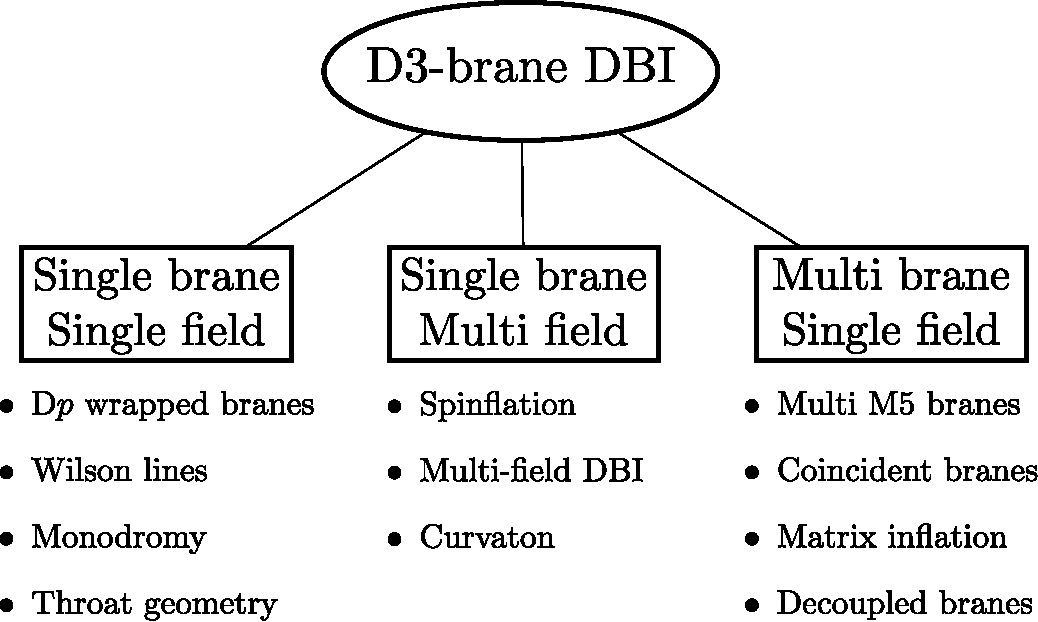
\includegraphics[keepaspectratio=true,
width=\textwidth]{./dbi/graphs/dbi-review.pdf}
 % dbi-review.pdf: 498x327 pixel, 72dpi, 17.57x11.54 cm, bb=0 0 498 327
 \caption{A schematic of recent DBI inspired models}
 \label{fig:review-dbi}
\end{figure}
% 

We have found that the standard DBI model appears to be in conflict with
observations. Many attempts have since been made to modify the original scenario in
order to evade these bounds. These can be classified according to
whether they involve single or multiple fields and single or multiple branes.
Figure~\ref{fig:review-dbi} shows a list of some models in
each category.


The most straightforward extensions of the DBI model have the same single degree of
freedom, but
rely on other physical mechanisms to ease the bounds on $r$.
A natural extension to the single ${\rm D3}$-brane model 
is to consider a ${\rm D}p$-brane wrapped around a $(p-3)$-cycle of the 
internal space.
This leads to a change in the relationship
between $\rho$ and $\vp$ from that defined in Section~\ref{sec:dbiinflation}
\cite{Kobayashi:2007hm, Becker:2007ui, Ward:2007gs}.  
For example, Becker \etal \cite{Becker:2007ui} 
have proposed a model in which inflation is driven by a warped ${\rm D5}$-brane. 
In this case, the range of allowed values for the inflaton 
becomes independent of the throat charge, $N$, which weakens the upper bound on 
the tensor-scalar ratio to $r \lsim 0.04$. (Strictly speaking there is a weak
dependence on the charge since $\Delta \varphi \sim N^{-1/4}$.)
However, in arriving at this bound, it was assumed that 
backreaction effects of any fluxes in the throat were 
negligible. 
Kobayashi \etal \cite{Kobayashi:2007hm} 
considered both ${\rm D5}$- and
${\rm D7}$ wrapped brane models, but concluded that the former case
required an excessively large background charge in 
order to relax the bounds on $r$. 
% 
This requirement is highly constraining, but is
still not as restrictive as the charge required by the single brane scenario,
which effectively rules that out as a predictive model. 
% 
Thus, wrapped brane configurations are preferable to
single brane models but the parameter space of the former is still severely
limited by the WMAP5 observations \cite{Alabidi:2008ej}. 
% However
% the difficulty in these models is that the backreaction is no longer under
% control. 


Another interesting proposal is warped Wilson line DBI. In this scenario, moduli
fields associated with Wilson
lines play the role of the inflaton \cite{Avgoustidis:2008zu}. This scenario is
T-dual to the
standard DBI model with non-parallel branes. In general, the model describes the
physics of a single brane with multiple position fields and multiple Wilson line
fields.
% 
However, in \Rref{Avgoustidis:2008zu} observational predictions were derived for
the case when the brane position is fixed and only one Wilson line degree of freedom
is used. This implementation is, therefore, a single brane, single field model.
% 
By following the method in Section~\ref{sec:upper-dbi} for this single field model,
a lower bound on $r$ is derived, instead of the upper bound \eqref{eq:upperbound}
\cite{Avgoustidis:2008zu}. The lower bound \eqref{eq:lowerbound} remains valid for
this scenario. 
% 
There are, therefore, two lower bounds on $r$ and the inconsistency of the
standard DBI model is not replicated. 
 


Changing the physical setting can also allow larger field ranges. Extremely large
field ranges can be achieved by considering
D4-branes in compactified manifolds containing monodromies. These large field
variations lead to possibly observable tensor modes
\cite{Silverstein:2008sg}. Although formulated in Type IIA string theory, the
monodromy model has a simple inflationary interpretation as a large field, slow roll
model with the potential $V(\vp)=\vp^{2/3}$. 


The next set of models that can be considered are the single brane, multi field
models. 
% 
The warped throat is six-dimensional, so it is natural to consider the case where
the D3-brane is not restricted to a radial trajectory. This was investigated in
Refs.~\cite{spinflation} and \cite{Huang:2007hh}. Increasing the degrees of
freedom in this way introduces the possibility of entropy mode production. There are
changes in the predictions for the amount and type of non-Gaussianity produced
and the constraints on $r$ can be eased \cite{Arroja:2008yy, Langlois:2009ej,
Langlois:2008qf, Langlois:2008wt, Mizuno:2009mv, Mizuno:2009cv}. 
% 
% Differences in
% the bi- and tri-spectra could enable multi-field DBI models to be distinguished
% from single field ones. In particular multi-field DBI models
% have a unique tri-spectrum term with amplitude proportional to $\fnlloc\fnleq$
% \cite{RenauxPetel:2009sj}. This opens the possibility of a distinct
% observational signature for this type of model.
% 
Other multi-field models introduce multiple copies of the single DBI action with
either
the same or different sound speeds \cite{Cai:2008if, Cai:2009hw},  use
different throat geometries \cite{Gmeiner:2007uw},
or apply the curvaton scenario \cite{Lyth:2001nq} to the DBI case
\cite{Li:2008fm, Kobayashi:2009cm}.

We have not yet addressed models with multiple branes but only one effective
degree of freedom. Multiple M5-branes in M-theory act with an effective single
degree of freedom but the Lyth bound is now significantly weakened and large
field ranges are possible \cite{Krause:2007jr}. It is also possible to consider
the case of $n$ coincident D3-branes in a warped throat \cite{thomasward, hltw,
Ward:2007gs}. In Chapter~\ref{ch:multibrane} we investigate this model in both
the large and small $n$ limits and show how the constraints derived in this
chapter can be applied.


% 
% 
% 
% % % % % % % % % % % % % % % % % % % % % % % % % % % % % % % % 
% =========================================================== %
\section{Discussion}
\label{sec:conclusion-dbi}
% =========================================================== %
% % % % % % % % % % % % % % % % % % % % % % % % % % % % % % % % 

In this chapter we have derived an upper limit on
the amplitude of the primordial gravitational wave spectrum
generated during UV DBI inflation. We considered   
the maximal inflaton field variation   
that can occur during the observable stages of inflation and assumed  
only that the brane was propagating inside the throat during that epoch. 
The bound (\ref{eq:upperbound}) is valid for an arbitrary inflaton potential and 
warp factor (modulo some weak caveats) and can be expressed 
entirely in terms of observable parameters once the volume of 
the five-dimensional sub-manifold of the throat has been specified. 
The inferred upper limit on $r$ is surprisingly strong. 
We find that the standard UV  
scenario predicts tensor perturbations that are undetectably small, 
at a level ${r_*} \, {\lsim} \, {10^{-7}}$. 

The current WMAP5 data 
favours models that generate a red spectral index $n_s<1$
when both the gravitational waves and running in the scalar 
spectral index are negligible. For UV versions of the scenario, 
we have identified a corresponding 
lower limit on $r$ which applies in this region of 
parameter space, $r_* \, \gsim \, 0.1 (1-n_s)$. It is clear that 
the standard scenario 
cannot satisfy both the upper and lower bounds 
on the tensor modes for the observationally favoured value 
$1-n_s \simeq 0.03$.


The generality of our 
analysis implies that modifying either the inflaton potential 
or the form of the warp factor is unlikely to resolve this discrepancy. 
On the other hand, there are a number of possible ways of reconciling  
theory with observation. In general, 
either the upper or lower limit on $r$ needs to be relaxed. 
Weakening the latter would require a violation of the slow-roll 
conditions or a blue spectral index. 
A value of $n_s >1$ is compatible with WMAP5 if the running of the 
spectral index 
is sufficiently negative, but is only marginally
consistent if just the tensor modes are non-negligible.  The 
upper limit on $r$ can be weakened by reducing 
the volume of $X_5$ or 
by generalizing the DBI action. Furthermore, it need not necessarily 
apply in IR versions of the scenario, although the BM bound will still hold
in such cases. 
We considered a generalized version of the 
DBI action and identified a necessary condition on the form of such  
an action for the BM bound to be relaxed.

% As a concrete example, 
% we investigated a version of IR inflation that is driven by 
% multiple coincident branes and found that  
% the bounds on the tensor-scalar ratio can indeed 
% be made compatible if the brane charges satisfy appropriate 
% conditions.   





In conclusion therefore, we have shown that primordial gravitational wave constraints 
combined with cosmological observations of the density perturbation
spectrum act as a powerful discriminant of DBI inflationary models. 
They also serve as an important observational guide for identifying viable 
generalizations of the scenario. In Chapter~\ref{ch:multibrane} we will explore
one particular generalisation, the multiple co-incident brane scenario
introduced in \Rref{thomasward}.
